\section{Electronic schematics}
% Powerboard
%\subsection{Powerboard}
\label{Schematics_Power}
\begin{figure}[!ht]
	\begin{center}
		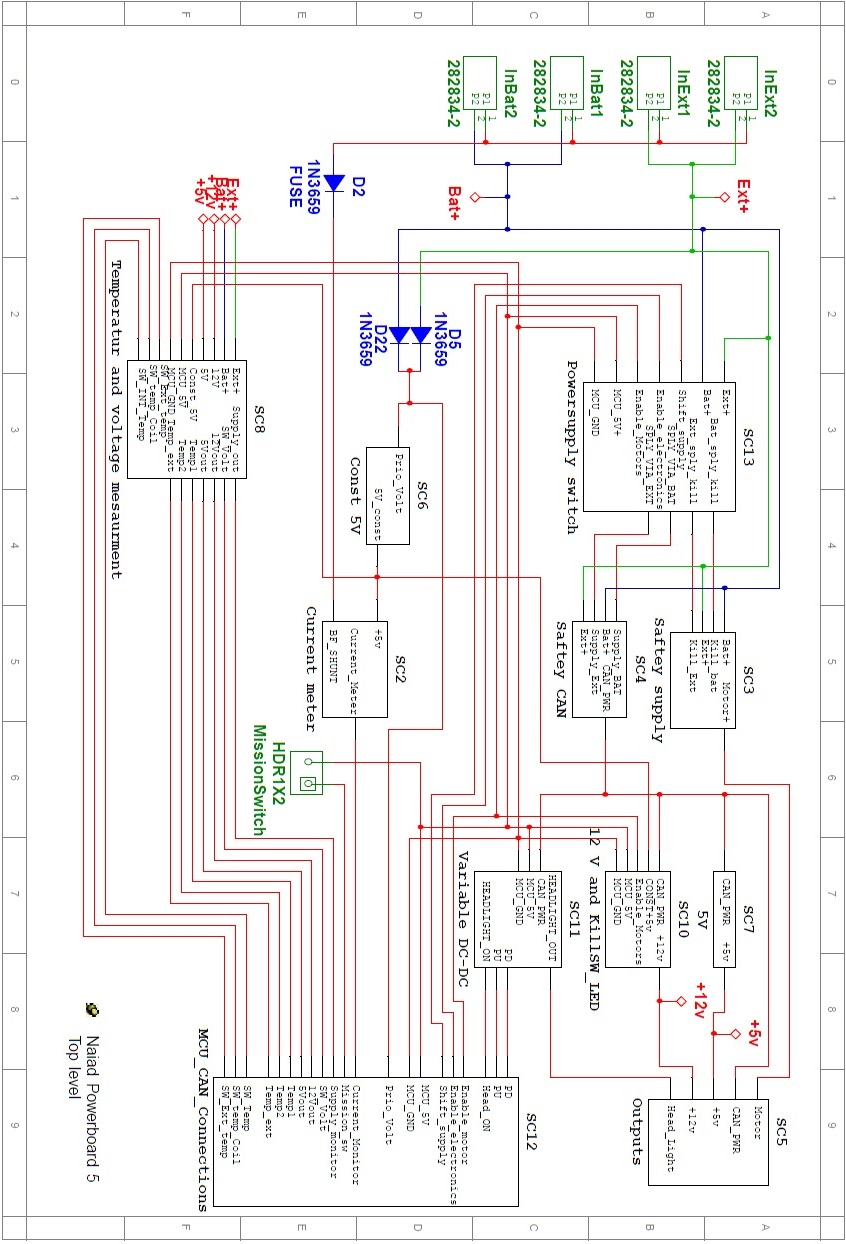
\includegraphics[width=13.2cm]{./Images/Powerboard_Scematics/Toplevel.jpg}
		\caption{Topview of Powerboard}
	\end{center}
\end{figure}

\begin{figure}[!ht]
	\begin{center}
		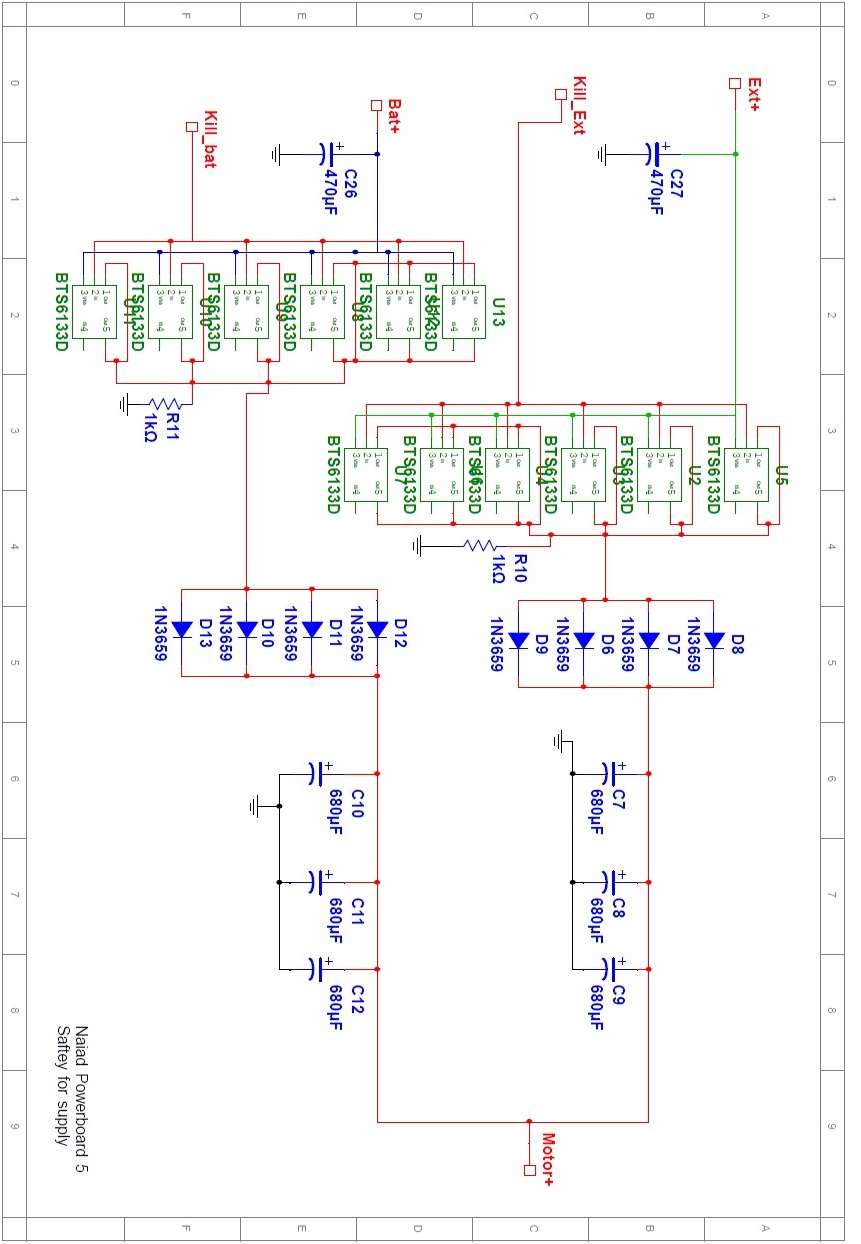
\includegraphics[width=13.2cm]{./Images/Powerboard_Scematics/Saftey_supply.jpg}
		\caption{Saftey for supply on Powerboard}
	\end{center}
\end{figure}

\begin{figure}[!ht]
	\begin{center}
		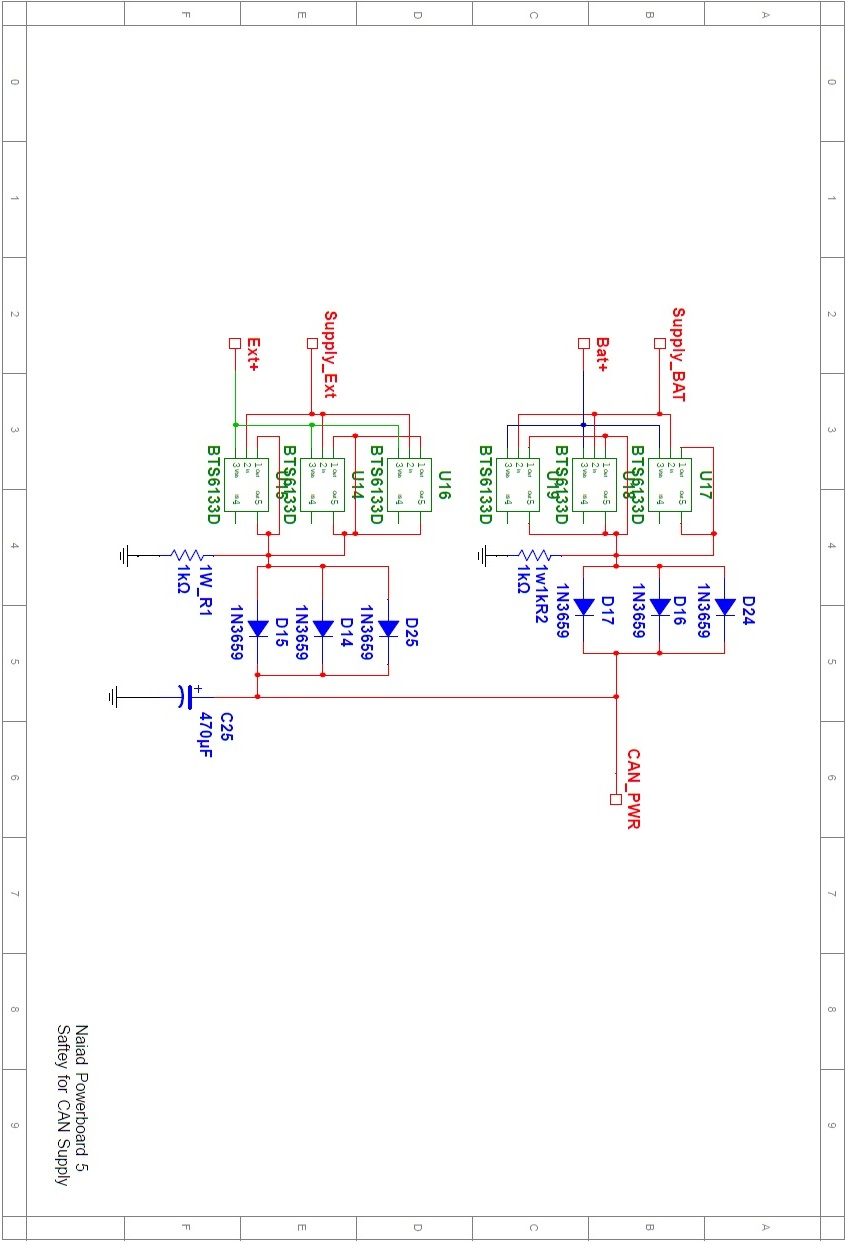
\includegraphics[width=13.2cm]{./Images/Powerboard_Scematics/Saftey_CAN.jpg}
		\caption{Saftey for CAN bus for Powerboard}
	\end{center}
\end{figure}

\begin{figure}[!ht]
	\begin{center}
		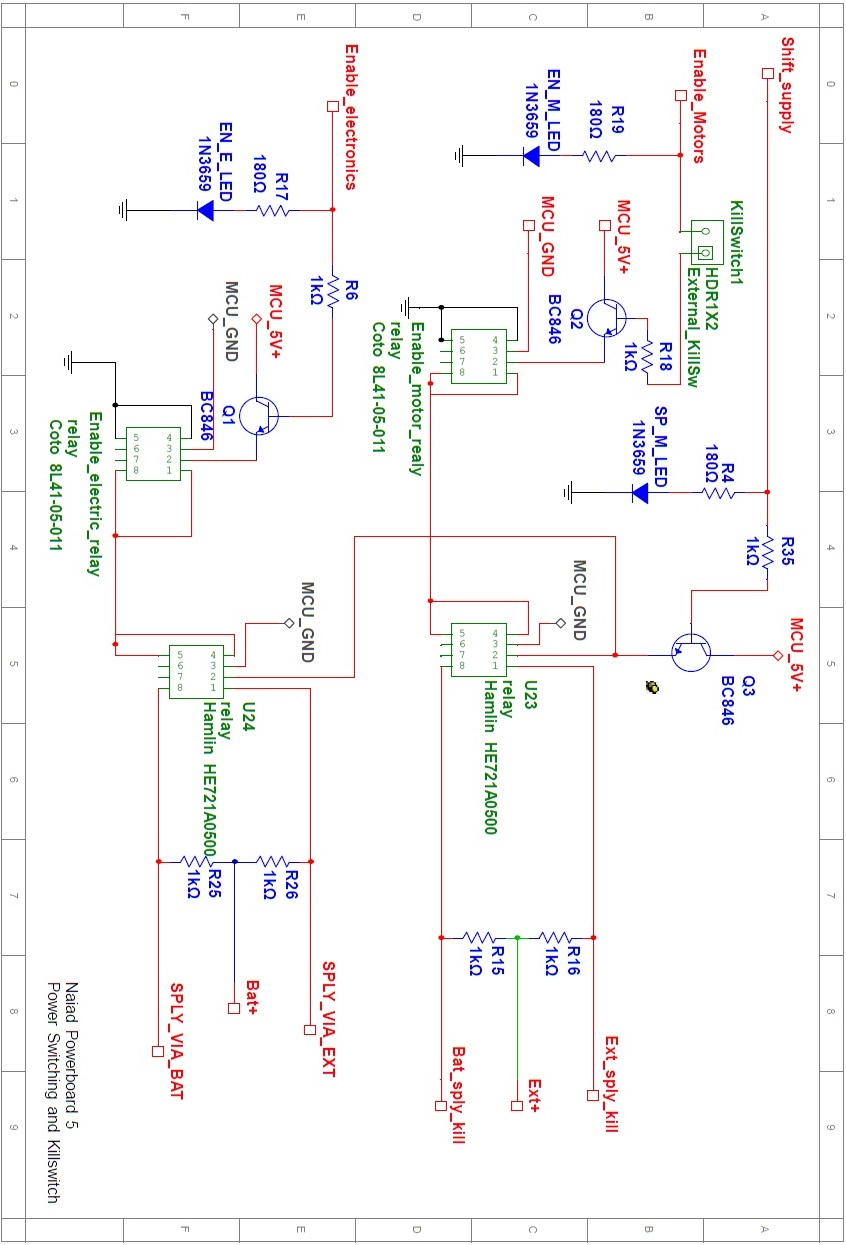
\includegraphics[width=13.2cm]{./Images/Powerboard_Scematics/Switching.jpg}
		\caption{Control what supply to use and kill switch Powerboard}
	\end{center}
\end{figure}

\begin{figure}[!ht]
	\begin{center}
		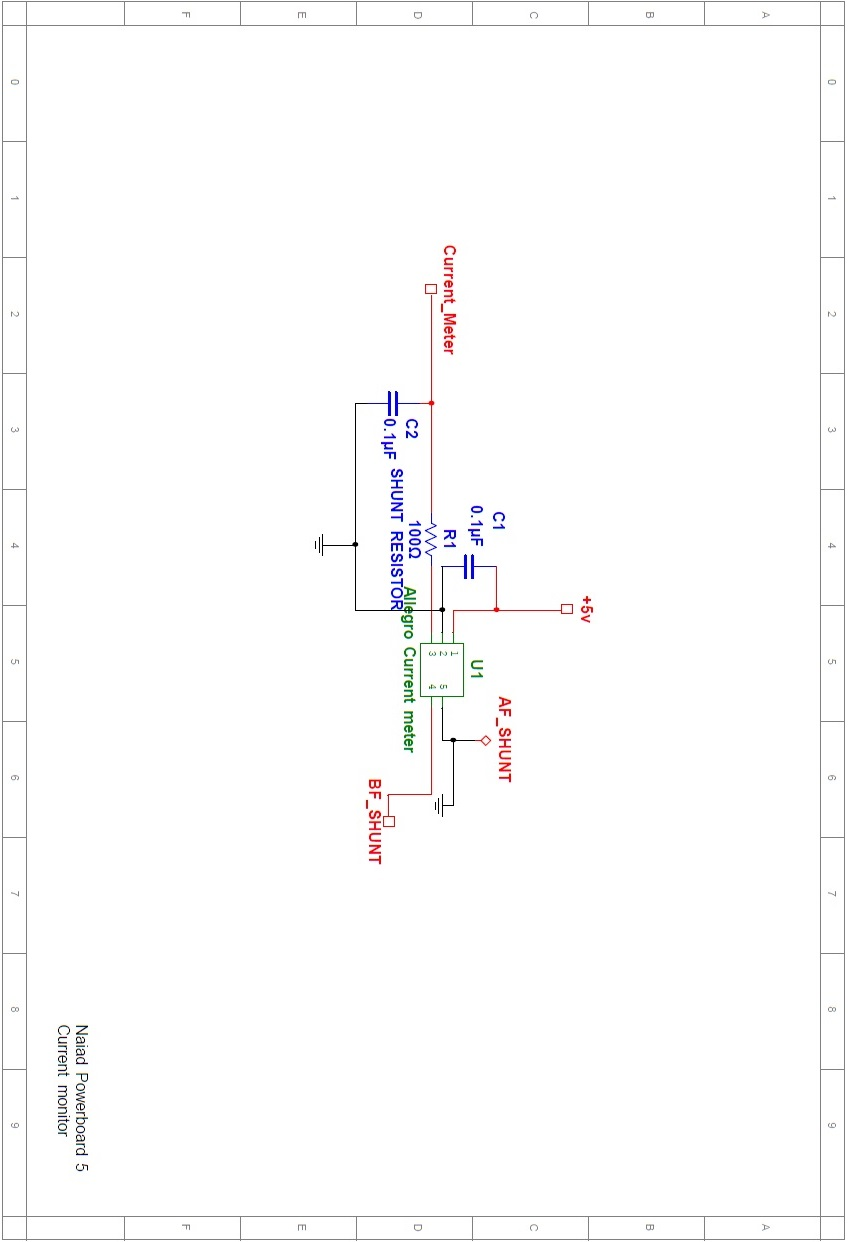
\includegraphics[width=13.2cm]{./Images/Powerboard_Scematics/Current_monitor.jpg}
		\caption{Current sensor to detect how much power the system use}
	\end{center}
\end{figure}

\begin{figure}[!ht]
	\begin{center}
		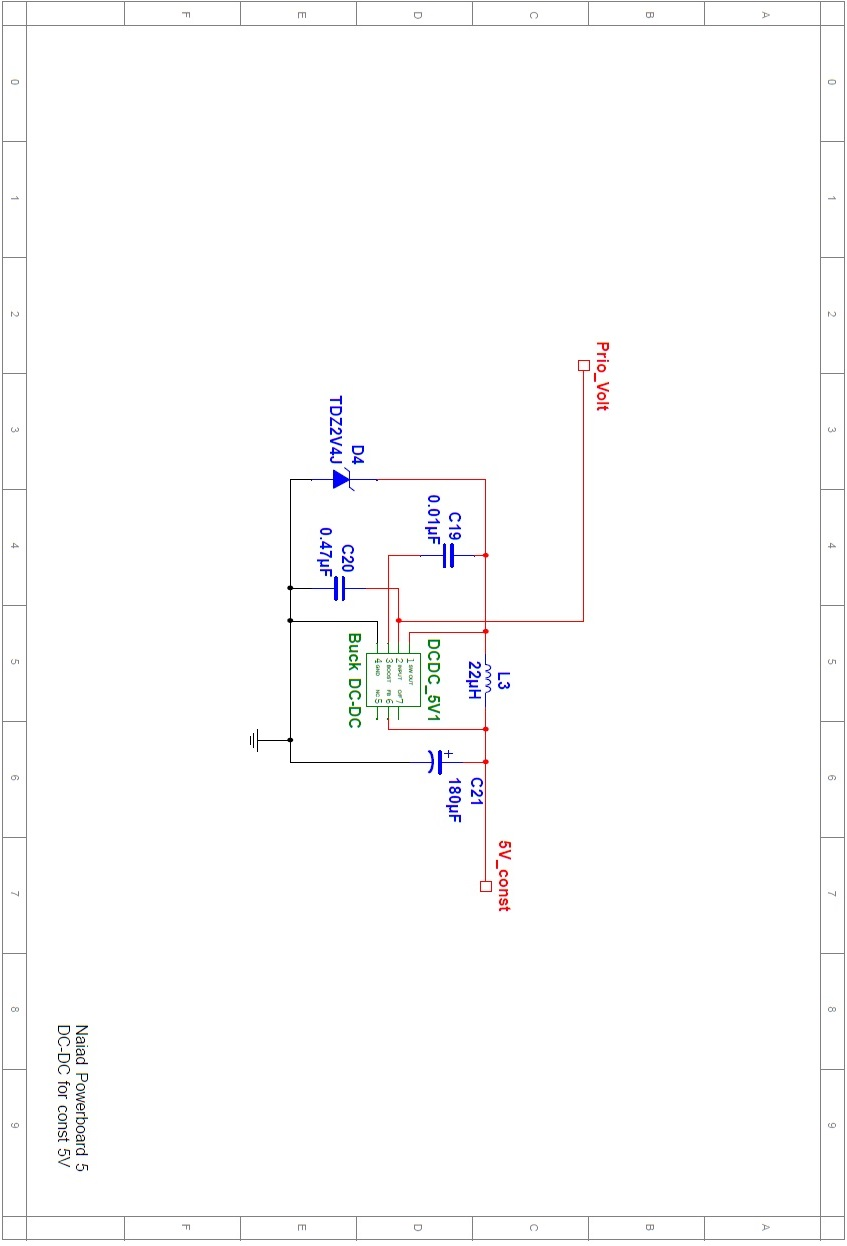
\includegraphics[width=13.2cm]{./Images/Powerboard_Scematics/5_const.jpg}
		\caption{DC-DC for the constant 5V trace on Powerboard}
	\end{center}
\end{figure}

\begin{figure}[!ht]
	\begin{center}
		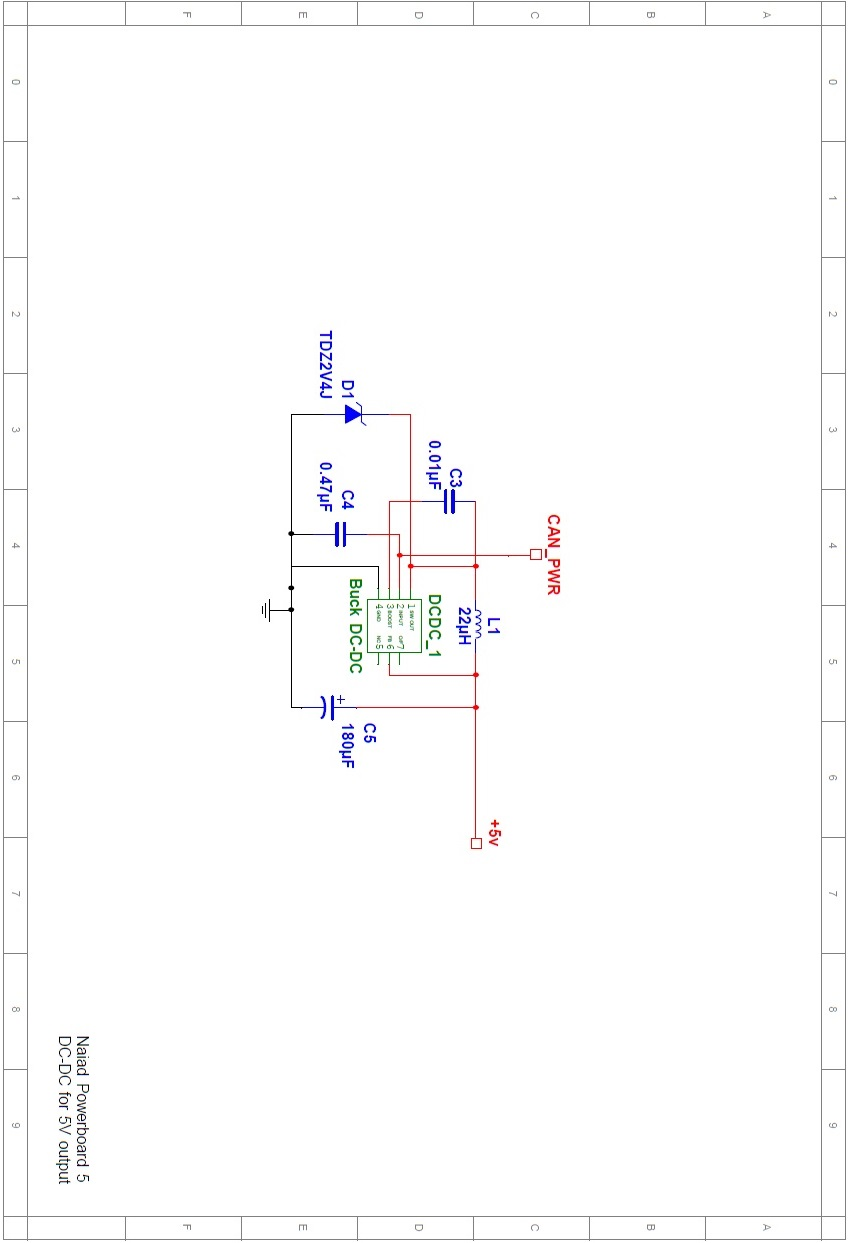
\includegraphics[width=13.2cm]{./Images/Powerboard_Scematics/5_out.jpg}
		\caption{DC-DC for the 5V output on Powerboard}
	\end{center}
\end{figure}

\begin{figure}[!ht]
	\begin{center}
		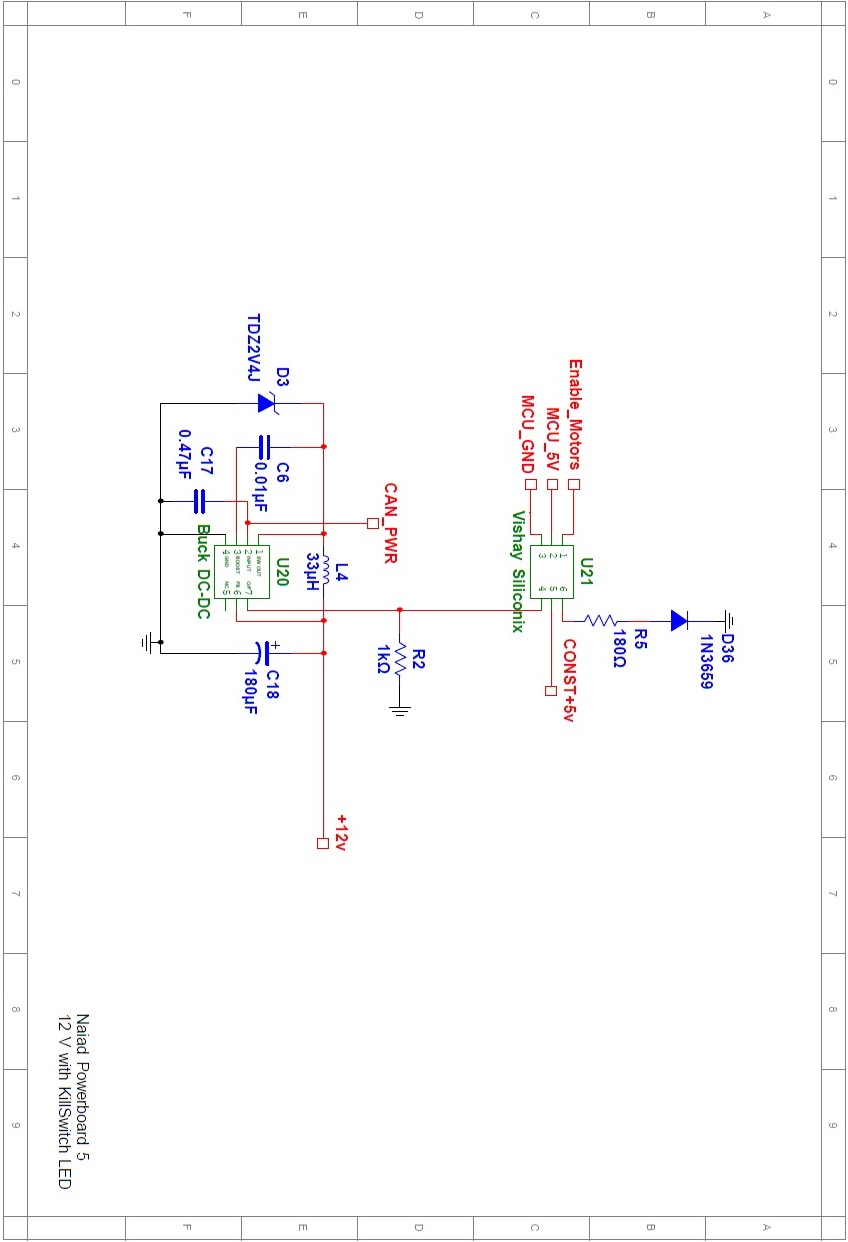
\includegraphics[width=13.2cm]{./Images/Powerboard_Scematics/12V.jpg}
		\caption{DC-DC for the 12V output on Powerboard}
	\end{center}
\end{figure}

\begin{figure}[!ht]
	\begin{center}
		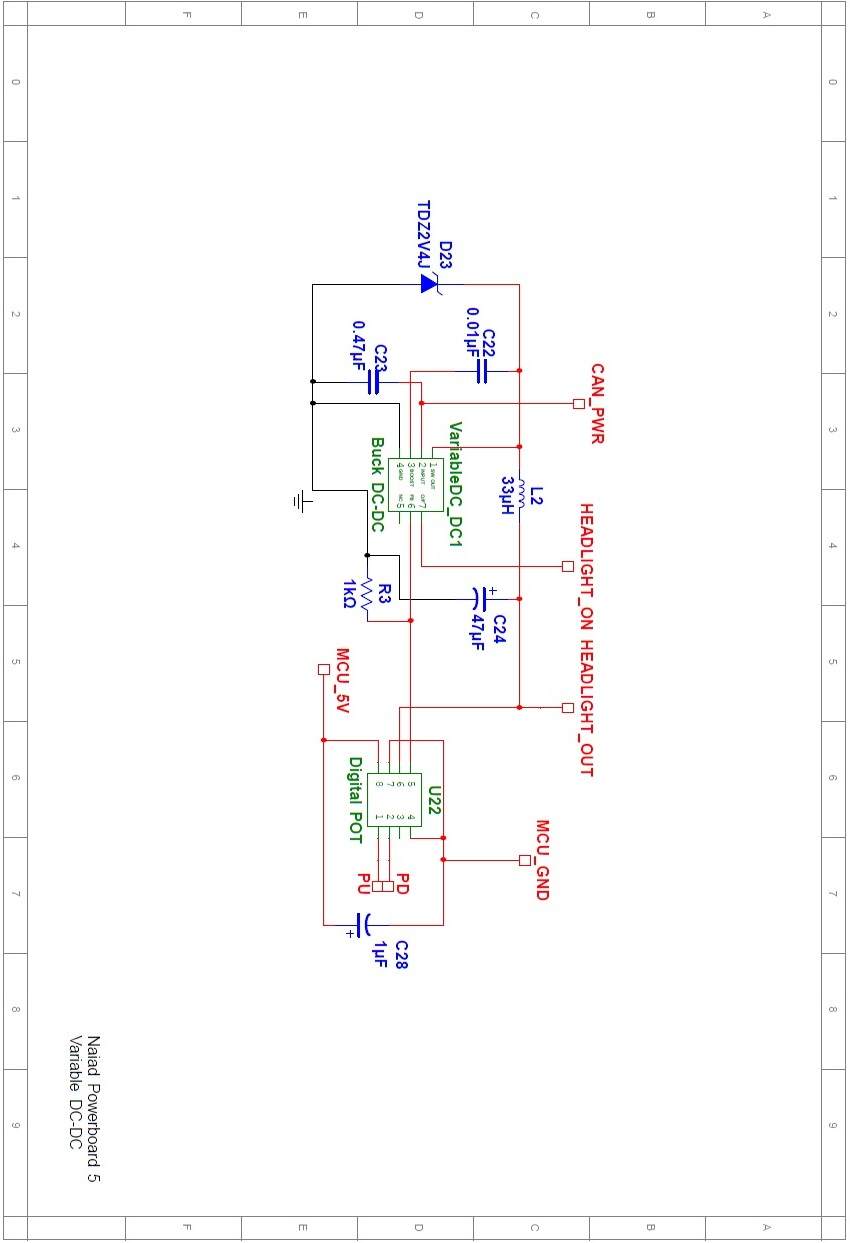
\includegraphics[width=13.2cm]{./Images/Powerboard_Scematics/Variable.jpg}
		\caption{DC-DC for the variable output on Powerboard}
	\end{center}
\end{figure}

\begin{figure}[!ht]
	\begin{center}
		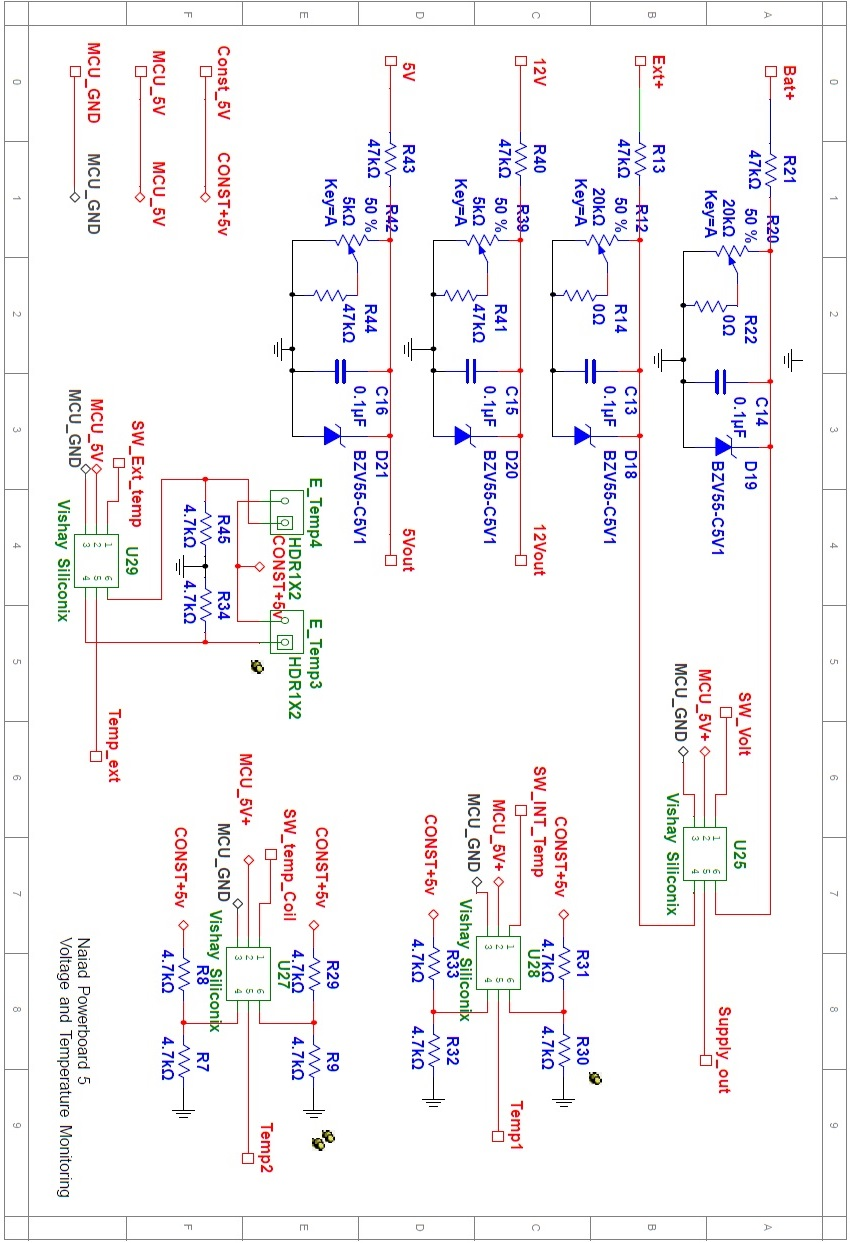
\includegraphics[width=13.2cm]{./Images/Powerboard_Scematics/monitor.jpg}
		\caption{Voltage and temperature monitor for Powerboard}
	\end{center}
\end{figure}

\begin{figure}[!ht]
	\begin{center}
		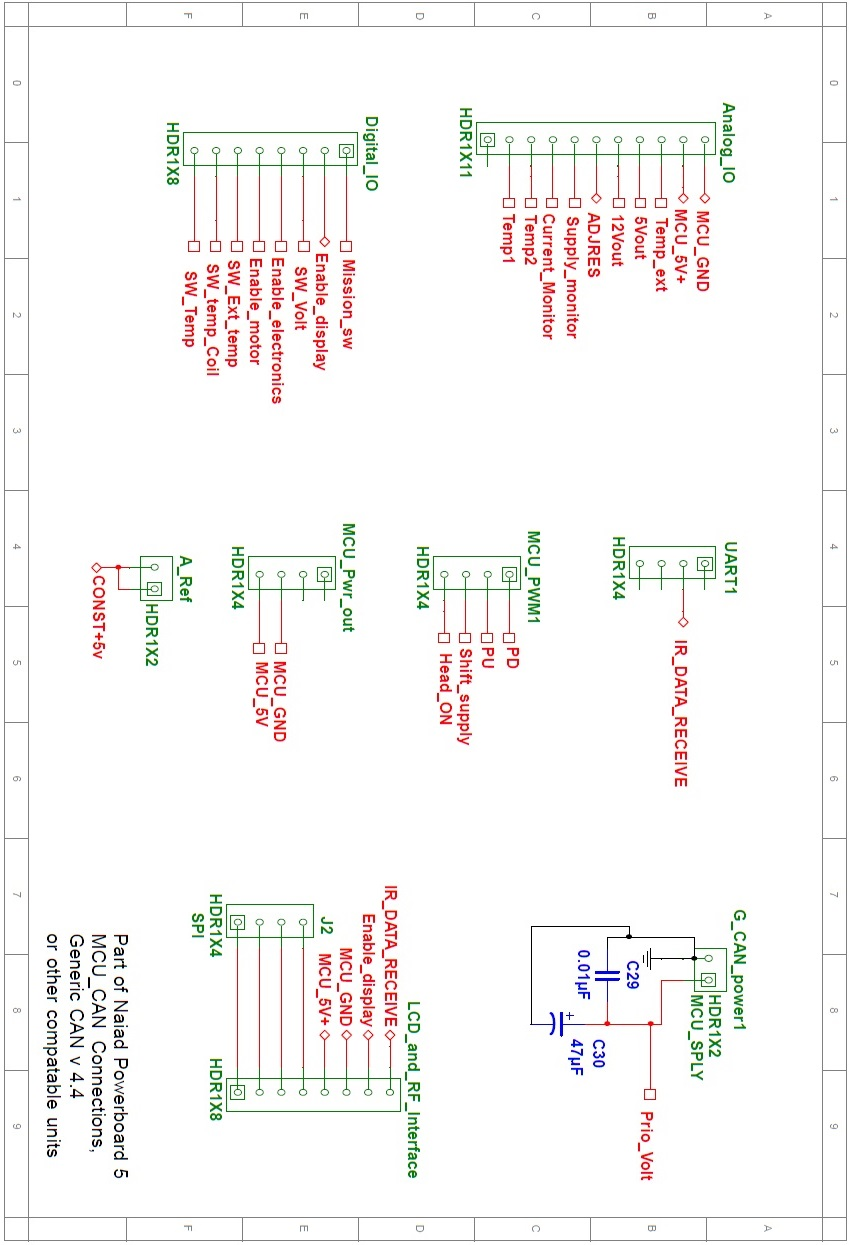
\includegraphics[width=13.2cm]{./Images/Powerboard_Scematics/MCU_CAN.jpg}
		\caption{Connection with MCU CAN card on Powerboard}
	\end{center}
\end{figure}

\begin{figure}[!ht]
	\begin{center}
		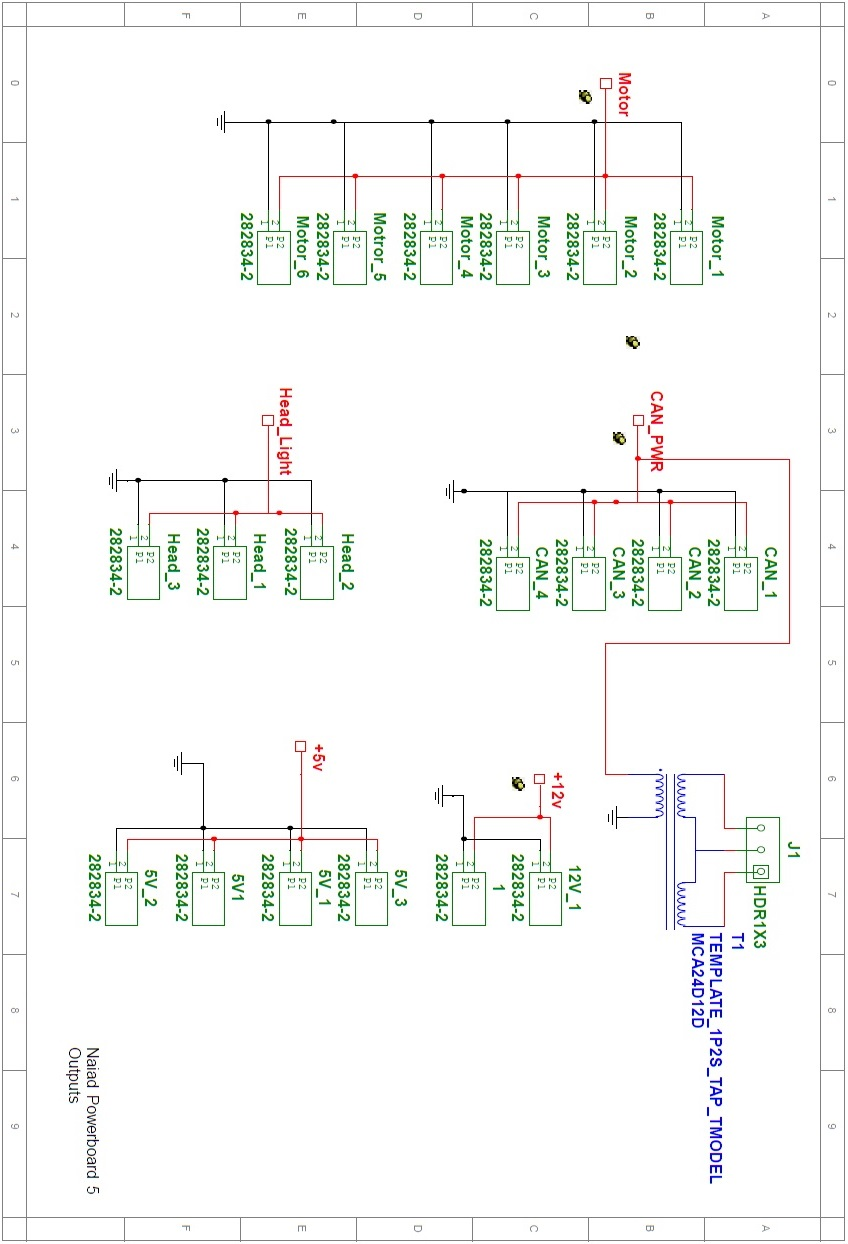
\includegraphics[width=13.2cm]{./Images/Powerboard_Scematics/Outputs.jpg}
		\caption{Outputs on Powerboard}
	\end{center}
\end{figure}

%\subsection{CAN 4.4}

\begin{figure}[!ht]
	\begin{center}
		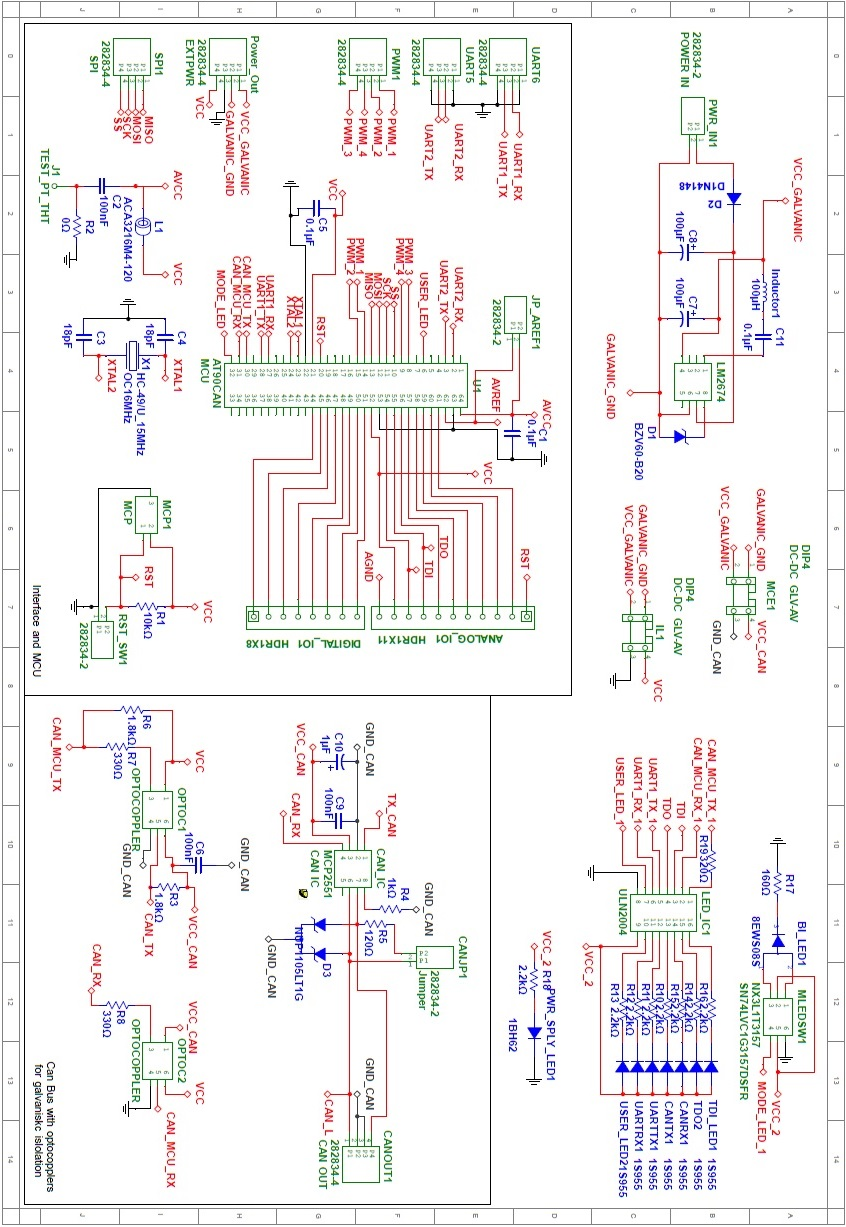
\includegraphics[width=13.2cm]{./Images/Powerboard_Scematics/Can_4.4.jpg}
		\caption{Generic CAN-card 4.4}
	\end{center}
\end{figure}


%\subsection{Speedlogger sensor}

%\subsection{Speedlogger Control}

\begin{figure}[!ht]
	\begin{center}
		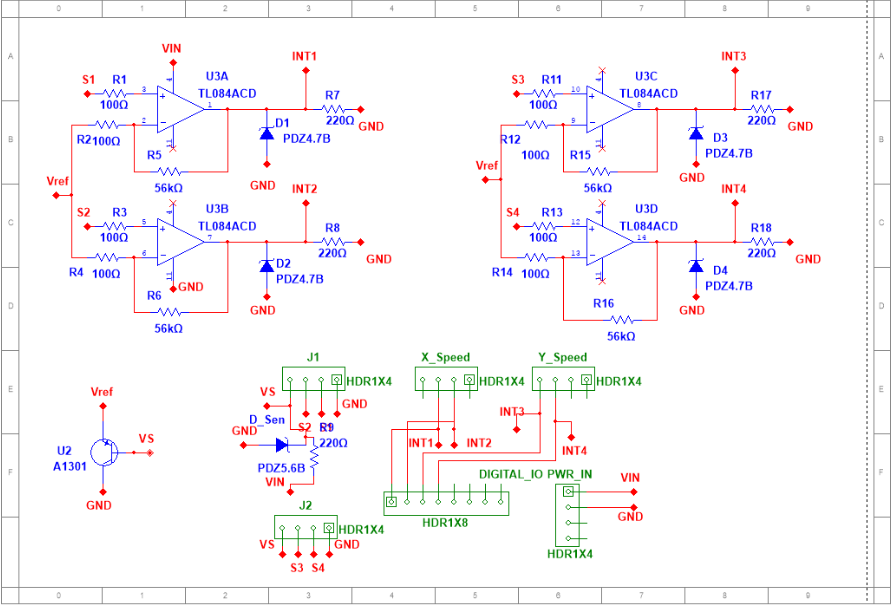
\includegraphics[width=\textwidth]{./Images/Powerboard_Scematics/SL_Shield_v1.2.png}
		\caption{Speedlogger sensor card}
	\end{center}
\end{figure}

%\subsection{INS-board} 

\begin{figure}[!ht]
	\begin{center}
		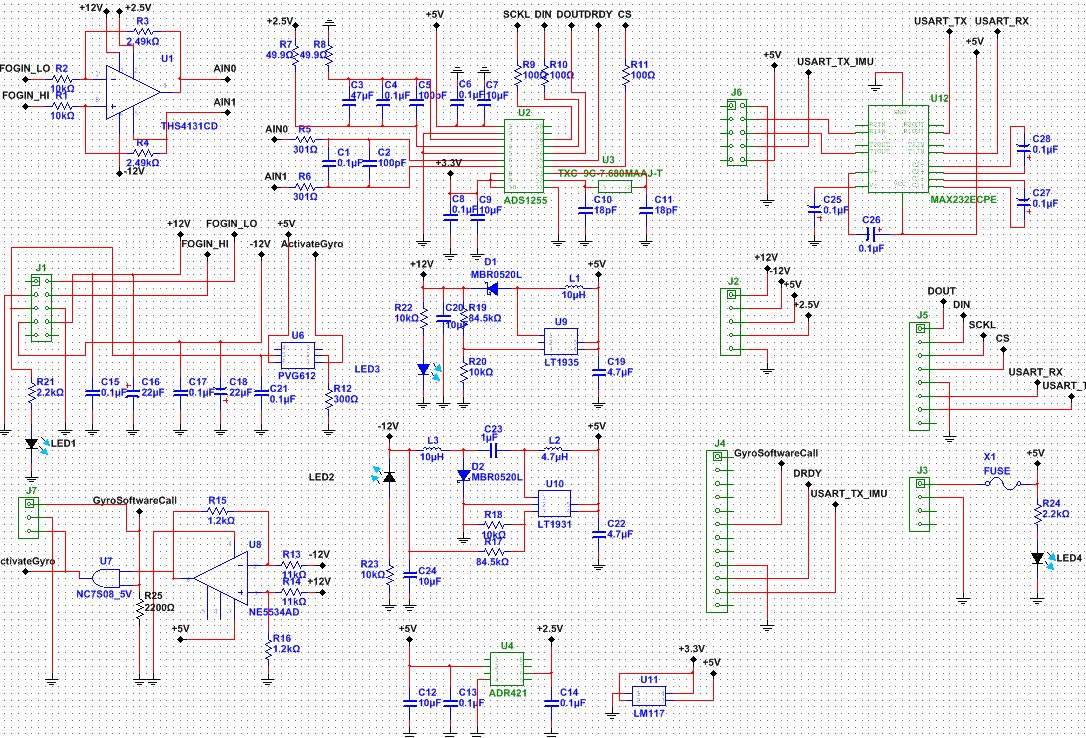
\includegraphics[width=\textwidth]{./Images/Powerboard_Scematics/INS_schematics.png}
		\caption{Speedlogger sensor card}
	\end{center}
\end{figure}

%\subsection{Sensor shield} 

%\subsection{LED shield}
 \begin{figure}[!ht]
	\begin{center}
		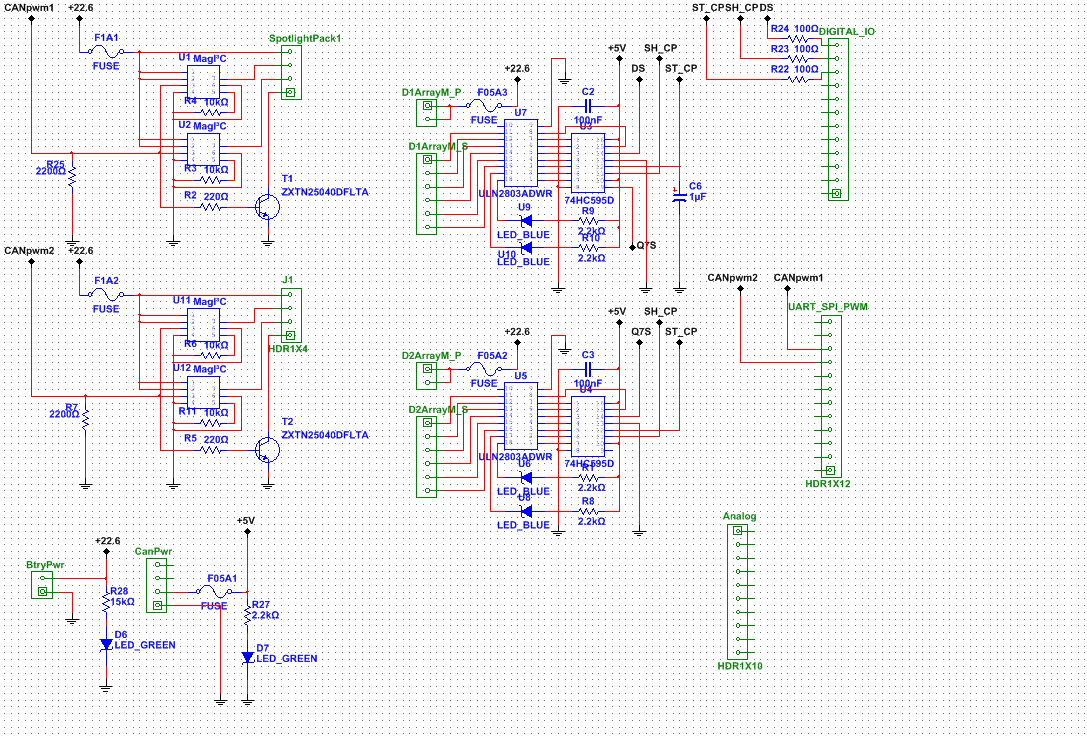
\includegraphics[width=\textwidth]{./Images/Powerboard_Scematics/LED_schematics.png}
		\caption{LEDcontrol-board}
	\end{center}
\end{figure}

%\subsection{Speedlogger} 